\documentclass[fleqn]{beamer}
 
 
\usepackage{dsfont}
\usepackage[utf8]{inputenc} 
\usepackage[T1]{fontenc}
\usepackage{lmodern}
\usepackage{graphicx}
\usepackage{units}
\usepackage{amsmath}
\usepackage{array}
\usepackage{textcomp}
\usepackage{biblatex}
\usepackage{stmaryrd} 
\usepackage{enumerate}
\usepackage{amsmath}
\usepackage{amsthm}
\usepackage{mathrsfs}
\usepackage{relsize}

\usetheme{CambridgeUS}

\newcommand\norm[1]{\left\lVert#1\right\rVert}

\setbeamertemplate{itemize subitem}[triangle] 
\setbeamertemplate{itemize subsubitem}[circle]
 
\begin{document}
\title{Automatic Calibration of Large Traffic Models}
\date{August $27^{th}$, 2015}
\author[Meziere, Gomes]{Felix Meziere \thanks{Ecole polytechnique [felix.meziere@polytechnique.edu]} \and Gabriel Gomes \thanks{University of California Berkeley [gomes@path.berkeley.edu]}}
\institute[PATH]{California PATH Program}
\maketitle
 
\begin{frame}
\frametitle{Introduction}
\framesubtitle{and motivation of this work}
\begin{itemize}
	\item Calibrate large traffic models input:
	\begin{itemize}
		\item Constants of the scenario
		\item Source and sink flows depending on day of week \& moment of year
	\end{itemize}	
	\item for the output to match:
	\begin{itemize}
		\item Congestion
		\item VMT and VHT
		\item Credible ramp flows
	\end{itemize}
	\item Goal: model accurately a usual traffic situation to make predictions.
\end{itemize}
\end{frame}

\begin{frame}
	\frametitle{Setup}
	\framesubtitle{Freeway and traffic model, data, notation}
	\begin{center}
		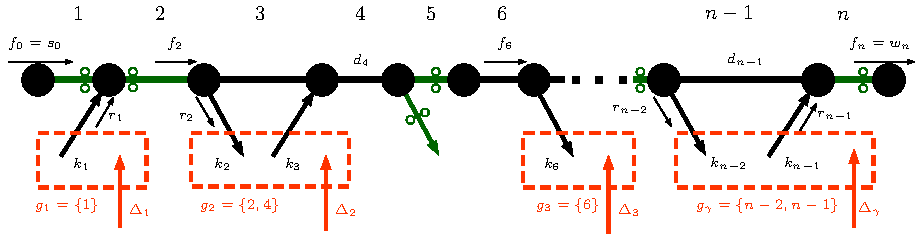
\includegraphics[width=4.5in]{figures/presentation_scheme.pdf}
	\end{center}
	\scriptsize{\begin{tabular}{llll}
		$M=\llbracket 1,n \rrbracket$ & Mainline link indexes  & $(f_{i})_{i\in{M}}$ & Mainline links exit flows\\
		$R\subset{M}$ & Ramp link indexes & $(d_{i})_{i\in{M}}$ & Mainline links densities\\
		$T\subset{M}$ & Monitored mainline links & $(r_{i})_{i\in{R}}$ & Ramps exit flows\\
		$K\subset{R}$ & Non-Monitored ramps & $\{\bar{f}_{0};(\bar{r}_{i})_{i\in{R}}\} $ & Flows inputted to the model\\
		$G=(g_{i})_{i\in{\llbracket 1,\gamma \rrbracket}}$ & Knob group indexes  & $(\widetilde{f}_{i})_{i\in{T}}$ & Measured mainline exit flows\\
		$\vec{k}=(k_{i_{1}},k_{i_{2}}...,k_{i_{\kappa}})$ & Knobs value vector & $(\widetilde{d}_{i})_{i\in{T}}$ & Measured mainline densities\\
		$\sigma=(\sigma_{i_{1}},\sigma_{i_{2}}...,\sigma_{i_{\kappa}})$ & on/off-ramp indicator & $(\widetilde{r}_{i})_{i\in{(R\backslash K)}}$ & Measured ramps exit flows\\
	\end{tabular}} 
\end{frame}

%\begin{frame}
%	\frametitle{Setup}
%	\framesubtitle{Context : PeMS data for 210E}
%	\begin{itemize}
%	\item Average of 5 Tuesdays in fall 2014
%	\item Flow, density and speed on 74 links every 5 minutes for 24 hours
%	\item Sensors (having deleted partial or too biased):
%	\begin{itemize}
%	\item 33/135 Mainline links are monitored
%	\item 26/28 On-ramps are monitored
%	\item 15/25 Off-ramps are monitored
%	\end{itemize}
%	\item Assumptions : uncertainty from sensor sensibility and bias
%	\begin{itemize}
%	\item Daily local flow uncertainty on mainline sensors : $I^{local}\approx10\%.[Average\ of\ mainline\ flow]$
%	\item Daily global uncertainty (on measures summed over the whole freeway): $I^{global}\approx5\%.[Global\ measure\ value]$
%	\end{itemize}
%	\end{itemize}
%\end{frame}

%\begin{frame}
%\frametitle{Setup}
%\framesubtitle{BeATS}
%Macroscopic freeway simulator
%\begin{itemize}
%\item Input:
%\begin{itemize}
%\item Topography of the freeway
%\item Fundamental Diagrams
%\item 5-min demands for sources and sinks ("split-ratios as output mode")
%\begin{itemize}
%\item As real data if the source or sink is monitored
%\item As a guessed template if not $\rightarrow$ need for 12 knobs
%\end{itemize}
%\end{itemize}
%\item Output: flow, densities and speeds on every link
%\item Run time: 5-8 seconds 
%\end{itemize}
%\end{frame}

\begin{frame}
	\frametitle{Constraints}
	\framesubtitle{Physical Boundaries}
	\begin{tabular}{l}
		Let $(t_{i}(t))_{i\in{K}}$ the templates:\\
		\\
		$m_{i}=\frac{[Capacity\ of\ ramp\ associated\ to\ k_{i}]}{\max_{t} t_{i}(t)}$\\
		\\
		\\
		\\
		$\forall i\in{K},\ \ \ \ \ 0\leq k_{i}\leq m_{i} \ \ \ \ \Leftrightarrow \ \ \ \ \ \vec{k}\in\mathscr{B}$
	\end{tabular}
\end{frame}


\begin{frame}
	\frametitle{Constraints}
	\framesubtitle{Knob groups and refined constraints}
		Each ramp is closely monitored by mainline sensors.\\
		\begin{equation*}
					\forall i \in \llbracket 1,\gamma \rrbracket, \ \ \ \ \ \ \ \Delta_{i} =\mathlarger{\sum\limits_{t\in \tau}}\bigg[\widetilde{f}_{\beta_{i}}(t)-\widetilde{f}_{\eta_{i}}(t)+\sum\limits_{j\in (R\backslash K)\cap S_{i}}\sigma_{j}.\widetilde{r_{j}}(t)\bigg]
		\end{equation*}
		~~~~~~~~~~~~~~~~...\\
		~~~~~~~~~~~~~~~~...\\
		~~~~~~~~~~~~~~~~...\\
		\begin{equation*}
			\centering
			\Leftrightarrow  \ \ \ \ \ \ \ \ \ \Delta_{i}=-\sum\limits_{j\in g_{i}}\sigma_{j}.k_{j}.\Theta
		\end{equation*}
\end{frame}


\begin{frame}
	\frametitle{Constraints}
	\framesubtitle{Loosening the constraints: uncertainty}
	\begin{itemize}
		\item $U^{mul}$, $U^{add}$ and $U^{global}$\\
		~\\
		\item $\forall i \in {\llbracket 1,\gamma \rrbracket}$, let the most permissive flow demands:\\
		~\\
		$\Delta_{i}^{-}=\max{\{|\Delta_{i}|-U^{add};|\Delta_{i}|.(1-U^{mul})\}}$\\
		$\Delta_{i}^{+}=\min{\{|\Delta_{i}|+U^{add};|\Delta_{i}|.(1+U^{mul})\}}$\\
		~\\
		\item Loosened constraints: 
			\begin{equation*}
			\forall i\in \llbracket 1,\gamma \rrbracket,\ \Delta_{i}^{-}\leq |\sum\limits_{j\in g_{i}}\sigma_{j}.k_{j}.\Theta| \leq \Delta_{i}^{+}
			\end{equation*}
	\end{itemize}

\end{frame}


\begin{frame}
	\frametitle{Performance and error calculation}
	\framesubtitle{Vehicles Hour Traveled (VHT)}
	\begin{itemize}
		\item Value computation from model output and data : 
		\begin{equation*}
				 VHT(\vec{k})=\frac{dt}{[1\ hour]}\sum_{i\in{T}}L_{i}\sum_{t\in \tau}d_{i}(t)
		\end{equation*}
		\item Error : 
		\begin{equation*}
			E_{VHT}(\vec{k})=\frac{|VHT(\vec{k})-\widetilde{VHT}|}{\widetilde{VHT}}
		\end{equation*}
	\end{itemize}
\end{frame}

\begin{frame}
	\frametitle{Performance and error calculation}
	\framesubtitle{Vehicles Mile Traveled (VMT)}
	\begin{itemize}
		\item Value computation from BeATS output and PeMS: 
		\begin{equation*}
			TVM(p)=\sum_{l\in{M}}\sum_{t}f^{(p)}_{l}(t)*length(l)
		\end{equation*}
		\item $\forall i\in{L}, f_{i}(midnight)\approx 0\Rightarrow$ TVM can be computed before BeATS:
		\begin{tabular}{l}
			Let $TVM^{ref}=TVM((1,...,1))$ outputed by BeATS\\
			\\
			\small{$TVM^{a\ priori}(k_{p})=TVM^{ref}+\sum_{i\in{K}}\biggl[\sigma_{i}.T_{i}.k_{i}.\sum_{j\in{M},j>i}length(j)\biggr]$}			
		\end{tabular}
		\item[$\rightarrow$] Same project \& penalize as KD, within $I^{global}$ :
		\begin{tabular}{l}
			minimize \small{$\ \ \ \ \ \norm{k_{p}-\underline{k_{p}}}_{2}$}\\
			s.t.\\
			\small{$TVM^{PeMS}.(1-I^{global})< TVM^{a\ priori}(k_{p})<TVM^{PeMS}.(1+I^{global})$}\\
			\small{$k_{p}\in{[k^{naMin},k^{naMax}]}$}\\
		\end{tabular}
		\item Relative difference : $\tau_{p}(TVM)=100* \frac{TVM^{BeATS}(p)-TVM^{PeMS}(p)}{TVM^{PeMS}(p)}$
	\end{itemize}
\end{frame}

\begin{frame}
	\frametitle{Performance and error calculation}
	\framesubtitle{Congestion Pattern matching (CP)}
	\begin{itemize}
		\item Principle : match the congested links and times into a box estimated from PeMS contour plot
		\item Error computation from BeATS output:
		\begin{itemize}
			\item A congestion treshold is defined for each mainline link :
			\begin{equation*} 
				\frac{Link\ capacity}{Link\ freeflow\ speed}+\delta
			\end{equation*}
			\item The number of pixels of the contour plot that are in the wrong state is the error:
			\begin{equation*}
				CP(p)=\sum_{t\in{\frac{24h}{dt}}}\sum_{l\in{L}}\mathds{1}_{wrong\ congestion\ state\ links}
			\end{equation*}
			\end{itemize}
		\item Relative difference : $\tau_{p}(CP)=100* \frac{CP(p)}{Total\ area\ of\ the\ boxes}$
	\end{itemize}
\end{frame}



\begin{frame}
	\frametitle{Problem Formulation}
	\framesubtitle{Optimization problem statement}
	\begin{itemize}
	\item qsd
	\end{itemize}
\end{frame}


\begin{frame}
	\frametitle{Numerical method}
	\framesubtitle{Requirements}
	\begin{itemize}
		\item Continuous search space: here, $\mathcal{S}=$12-D hypercube
		\item Function to minimize : mix of correlated and uncorrelated functions with non-differentiable congestion effects
		\item[$\rightarrow$]Continuous black-box imputation problem
	\end{itemize}
\end{frame}


\begin{frame}
	\frametitle{Numerical method}
	\framesubtitle{Covariance Matrix Adaptation - Evolution Strategy (CMA-ES)}
	\begin{itemize}
		\item Most powerful evolutionary algorithms for single-objective real-valued optimization (very used) 
		\item "Designed for difficult non-linear non-convex black-box optimisation problems in continuous domain"
		\item "Typically applied to unconstrained or bounded constraint optimization problems, and search space dimensions between three and a hundred"
		\item Does not presume existence of approximate gradients : feasible on our non-smooth problem
		\item \em Adaptive \em algorithm : almost no parameter tuning $\rightarrow$ suitable to be used on several different freeways and days.
		\item Time does not matter for this initial study : not the fastest ES but excellent solution quality 
		\item Principle : 12*12 covariance matrix adapts the stochastic sampling direction and step size on-the-go 	
	\end{itemize}
\end{frame}


\begin{frame}
	\frametitle{Numerical method}
	\framesubtitle{Constraints implementation (1)}
	For the single-knob groups, we can refine the knob boundaries using these two uncertainties as a limit:
\begin{equation*}
	\begin{split}
		k_{i}^{min}=max(\{min(\{\alpha.k_i^{*};k_{i}^{*}-\frac{I^{local}}{\sum_{t} t_{i}(t)}\});0\}) \\ 
		k_{i}^{max}=min(\{max(\{\beta.k_i^{*};k_{i}^{*}+\frac{I^{local}}{\sum_{t} t_{i}(t))}\});\mu_{i}\})
	\end{split}	
\end{equation*}
\end{frame}


\begin{frame}
	\frametitle{Numerical method}
	\framesubtitle{Constraints implementation (2)}
	\framesubtitle{Refined boundaries on multiple-knob groups}
Repairing : Here, we project the knobs of the group on a space delimited by the two "tolerance hyperplans" for $\Delta_{k}$:
\begin{tabular}{l}
\\
Let $\overline{k_{p}}$ the knobs vector to be evaluated at iteration p before projection\\
Let $J=\{j,card(g_{j}>1)\}$ and $\forall i\in{K},T_{i}=\sum_{t}t_{i}(t)$\\
\\
minimize $\ \ \ \ \ \norm{k_{p}-\overline{k_{p}}}_{2}$\\
s.t.\\
\small{$\forall j\in{J} \ \ min(\{\alpha.\Delta_{j};\Delta_{j}-I^{local}\})< \sum_{i\in{g_{j}}} \sigma_{i}.k_{i}.T_{i}<max(\{\beta.\Delta_{j};\Delta_{j}+I^{local}\})$}\\
\small{$k\in{[k^{naMin},k^{naMax}]}$}\\
\end{tabular}
\end{frame}


\begin{frame}
	\frametitle{Experiment settings}
	\framesubtitle{Data}
	\begin{itemize}
	\item qsd
	\end{itemize}
\end{frame}

\begin{frame}
	\frametitle{Experiment settings}
	\framesubtitle{Model and simulator}
	\begin{itemize}
	\item qsd
	\end{itemize}
\end{frame}


\begin{frame}
	\frametitle{Experiment settings}
	\framesubtitle{Implementation of congestion pattern}
	\begin{itemize}
	\item qsd
	\end{itemize}
\end{frame}


\begin{frame}
	\frametitle{Experiment results}
	\framesubtitle{General observations}
	\begin{itemize}
	\item qsd
	\end{itemize}
\end{frame}


\begin{frame}
	\frametitle{Experiment results}
	\framesubtitle{Typical execution}
	\begin{itemize}
	\item qsd
	\end{itemize}
\end{frame}



\begin{frame}
	\frametitle{Experiment results}
	\framesubtitle{Effect of $U^{mul}$}
	\begin{itemize}
	\item qsd
	\end{itemize}
\end{frame}



\begin{frame}
	\frametitle{Experiment results}
	\framesubtitle{Effect of $U^{add}$}
	\begin{itemize}
	\item qsd
	\end{itemize}
\end{frame}



\begin{frame}
	\frametitle{Experiment results}
	\framesubtitle{Effects of $\sigma$}
	\begin{itemize}
	\item qsd
	\end{itemize}
\end{frame}


\begin{frame}
	\frametitle{Experiment results}
	\framesubtitle{Effects of $\lambda$}
	\begin{itemize}
	\item qsd
	\end{itemize}
\end{frame}


\begin{frame}
	\frametitle{Further work}
	\framesubtitle{Next steps and ideas}
	\begin{itemize}
	\item qsd
	\end{itemize}
\end{frame}



\end{document}